\documentclass[ 12pt,a4paper,twocolumn,fleqn]{report}
\usepackage{graphicx}
\usepackage[a4paper,top=20mm, bottom=30mm, left=10mm, right=25mm]{geometry}
\usepackage{fancyhdr}
\usepackage{hyperref}
\usepackage{listings}
\usepackage[]{algorithm2e}
\usepackage{color}
\usepackage{fancybox}
\usepackage{lastpage}
\thisfancypage{%
  \setlength{\fboxsep}{20pt}\doublebox}{}
\pagestyle{fancy}
\usepackage{lineno}
\usepackage{xtab,booktabs}
\usepackage{setspace}
\usepackage{amsmath}
\usepackage{xcolor}
\usepackage{tocloft} % <================================================
\addtolength{\cftaftertoctitleskip}{-\baselineskip} % <=================
\usepackage[compact]{titlesec}
\titlespacing{\section}{0pt}{*0}{*0}
\titlespacing{\subsection}{0pt}{*0}{*0}
\titlespacing{\subsubsection}{0pt}{*0}{*0}
\setlength\columnsep{25pt}
\makeatletter
\g@addto@macro{\normalsize}{%
\setlength{\abovedisplayskip}{0pt}
\setlength{\abovedisplayshortskip}{0pt}
\setlength{\belowdisplayskip}{0pt}
\setlength{\belowdisplayshortskip}{0pt}}
\makeatother
\mathindent=0.0pt
\usepackage{float}
\renewcommand{\baselinestretch}{1.0}
\pagenumbering{global}
\fancypagestyle{myfooter}{
    \fancyhf{} % clear all header and footer fields
    \fancyfoot[L]{Department of CSE} % left footer
    \fancyfoot[R]{\protect\thepage} % right footer with \protect
    \renewcommand{\headrulewidth}{0pt} % remove header line
    \renewcommand{\footrulewidth}{0.4pt} % footer line width
}

% Redefine plain page style for chapters
\fancypagestyle{plain}{
    \fancyhf{} % clear all header and footer fields
    \fancyfoot[R]{\protect\thepage} % right footer with \protect
    \renewcommand{\headrulewidth}{0pt} % remove header line
    \renewcommand{\footrulewidth}{0pt} % remove footer line
}

% Define a new page style combining fancy and myfooter
\fancypagestyle{combined}{
    \fancyhf{} % clear all header and footer fields
    \fancyhead{} % clear header fields
    \fancyhead[L]{The Transformative Potential of SEMG and AI in
Neuromuscular Disease Detection} % fancy header content
    \fancyfoot[L]{Department of CSE (AI \& ML), SOE, DSU} % left footer
    \fancyfoot[R]{\protect\thepage} % right footer with \protect
    \renewcommand{\headrulewidth}{0.4pt} % header line width
    \renewcommand{\footrulewidth}{0pt} % footer line width
}
\begin{document}

\fancyfoot[R]{Page \thepage}  
\pagestyle{plain}
%\chead{}

\onehalfspacing
\onecolumn
\begin{center}
    \huge\textbf{DAYANANDA SAGAR UNIVERSITY} \\
    \large\textbf{Devarakaggalahalli, Harohalli,
Kanakapura Road,
Bengaluru South Dt. – 562 112 }
\end{center}
\begin{figure}[h]
    \centering
    
\includegraphics[width=0.4\textwidth]{image/SCHOOL OF ENGINEERING_c.png} % Adjust the file name and path as needed
\end{figure}
\begin{center}
    \Large\textbf{Bachelor of Technology} \\
    \normalsize\textbf{in} \\
    \large\textbf{COMPUTER SCIENCE AND ENGINEERING} \\
    \large\textbf{(ARTIFICIAL INTELLIGENCE AND MACHINE LEARNING)}
\end{center}
\begin{center}
\large\textbf{23AM3503- Natural Language Processing}\\
\end{center}
\begin{center}
    \large\textbf{A MiniProject Report On} \\
    \large\textbf{ Project Title}
\end{center}

\begin{center}
    \small\textbf{By} \\
    \normalsize\textbf{NAME - USN} \\
    \normalsize\textbf{NAME - USN} \\
    \normalsize\textbf{NAME - USN} \\
    \normalsize\textbf{NAME - USN} 

\end{center}
\begin{figure}[h]
    \centering
    
\includegraphics[width=0.11\textwidth]{image/Logo of AIML.jpg} % Adjust the file name and path as needed
\end{figure}
\begin{center}
    \normalsize\textbf{Under the supervision of} \\
    \normalsize\textbf{Faculty Name} \\
    \normalsize\textbf{Designation}\\
    \normalsize\textbf{Computer Science \& Engineering (AI \& ML)}
\end{center}
\vfill
\begin{center}

    %\normalsize\textbf{DEPARTM%ENT OF COMPUTER SCIENCE \& ENGINEERING} \\
    %\normalsize\textbf{(ARTIFICIAL INTELLIGENCE AND MACHINE LEARNING)} \\
   % \vspace{5mm}
    \normalsize\textbf{SCHOOL OF ENGINEERING} \\
    %\normalsize\textbf{DAYANANDA SAGAR UNIVERSITY} \\
   % \vspace{2mm}
   \normalsize\textbf{(2025 -- 2026)}
\end{center}



\newpage
  \pagestyle{plain}
\thisfancypage{%
  \setlength{\fboxsep}{20pt}\doublebox}{}
\begin{center}

\vspace{2mm}

\includegraphics[width=1\textwidth]{image/certificate.png} \\
\begin{center}
    \textcolor{blue}{\LARGE\textbf{{DAYANANDA SAGAR UNIVERSITY}}} \\
    \large\textbf{Department of Computer Science \& Engineering}\\
    \large\textbf{(ARTIFICIAL INTELLIGENCE AND MACHINE LEARNING)}\\
    \small\textbf{Devarakaggalahalli, Harohalli,
Kanakapura Road,
Bengaluru South Dt. – 562 112\\}
    \small\textbf{Karnataka, India}
\end{center}
\vspace{10mm}
\Large{\underline{\textbf{CERTIFICATE}}} \\
  \end{center}
  \vspace{10mm}
\normalsize
This is to certify that the project entitled \textbf{“Project Title”} is carried out by \textbf{NAME(USN), NAME(USN), NAME(USN), NAME(USN)}, 
bonafide students of Bachelor of Technology in Computer Science and Engineering at the School of Engineering, Dayananda Sagar University, Bangalore, in partial fulfillment for the award of a degree in Bachelor of Technology in Computer Science and Engineering, during the year 
\textbf{2025 \-- 2026}.\\



%\noindent
\vspace{10mm}

\begin{minipage}[t]{0.31\textwidth}
\small
  \textbf{Course Handling faculty}\\
  Designation\\
  Dept. of CSE (AI\&ML)\\
  School of Engineering\\
  Dayananda Sagar University\\
  \\
  Signature .........................\\
\end{minipage}%
\hfill
\begin{minipage}[t]{0.31\textwidth}
\small
  \textbf{Prof. Pradeep Kumar K}\\
  Course Co-ordinator\\
  Dept. of CSE (AI\&ML)\\
  School of Engineering\\
  Dayananda Sagar University\\
  \\
  Signature .........................\\
\end{minipage}%
\hfill
\begin{minipage}[t]{0.34\textwidth}
\small
  \textbf{Dr. Jayavrinda Vrindavanam}\\
  Professor \& Chairperson\\
  Dept. of CSE (AI\&ML)\\
  School of Engineering\\
  Dayananda Sagar University \\
  \\
  Signature .........................\\
\end{minipage}



\newpage
  \pagestyle{plain}
\thisfancypage{%
  \setlength{\fboxsep}{20pt}\doublebox}{}
  \begin{center}
    \huge\textbf{DECLARATION}
\end{center}
\vspace{15mm}
We, \textbf{NAME(USN),NAME(USN), NAME(USN),NAME(USN) } are students of the seventh semester B.Tech in Computer Science and Engineering (AI \& ML) at the School of Engineering, Dayananda Sagar University. We hereby declare that the Mini Project titled \textbf{“Project Title”} has been carried out by us and submitted in partial fulfillment for the award of a degree in \textbf{Bachelor of Technology} in \textbf{Computer Science and Engineering} during the academic year \textbf{2025--2026}.
\vspace{15 mm}


\noindent
\begin{minipage}{0.8\textwidth}
    \textbf{Student:} \hfill\textbf{Signature}\\
    
    \textbf{Name 1:} NAME\\ \textbf{USN:} USN \\
    
    \textbf{Name 2:} NAME \\ \textbf{USN:} USN \\
    
    \textbf{Name 3:} NAME \\ \textbf{USN:} USN \\
    
    \textbf{Name 4:} NAME \\ \textbf{USN:} USN \\

\end{minipage}

\begin{flushleft}
    \textbf{Place:} Bangalore \\
    \textbf{Date:} 
\end{flushleft}


\newpage
  \pagestyle{plain}
\thisfancypage{%
  \setlength{\fboxsep}{20pt}\doublebox}{}
\begin{center}
\huge\textbf{ACKNOWLEDGEMENT}
\end{center}
\vspace{15mm}
\normalsize
It is a great pleasure for us to acknowledge the assistance and support of many individuals who have been responsible for the successful completion of this project work.
First, we take this opportunity to express our sincere gratitude to School of Engineering\& Technology, Dayananda Sagar University for providing us with a great opportunity to pursue our Bachelor’s degree in this institution.
\\
\hfill
\\
We would like to thank \textbf{ Dr. Udaya Kumar Reddy K R, Dean, School of Engineering \&
Technology, Dayananda Sagar University }for his constant encouragement and expert advice.
It is a matter of immense pleasure to express our sincere thanks to\textbf{ Dr. Jayavrinda
Vrindavanam, Department Chairman, Computer Science and Engineering (Artificial
Intelligence and Machine Learning), Dayananda Sagar University}, for providing right academic guidance that made our task possible.
\\
\hfill
\\
We would like to thank our guide  \textbf{NAME, Designation, Dept. of
Computer Science and Engineering of Artificial Intelligence and Machine Learning, Dayananda Sagar University} for sparing his valuable time to extend help in every step of our
project work, which paved the way for smooth progress and the fruitful culmination of the project.
\\
\hfill
\\
We would like to thank our \textbf{Course Coordinator Prof. Pradeep Kumar K} as well as all the staff members
of Computer Science and Engineering (AI\& ML) for their support.
We are also grateful to our family and friends who provided us with every requirement
throughout the course.
We would like to thank one and all who directly or indirectly helped us in the Project work


\newpage
  \pagestyle{fancy}
\thisfancypage{%
  \setlength{\fboxsep}{20pt}\doublebox}{}
\tableofcontents{\protect\enlargethispage*{\baselineskip}}

\newpage
  \pagestyle{fancy}
\thisfancypage{%
  \setlength{\fboxsep}{20pt}\doublebox}{}
\begin{center}
\huge\textbf{LIST OF FIGURES}
\end{center}
\vspace{15mm}
\begin{center}
    \begin{tabular}{|c|c|c|}
     \hline
     Fig .Number & Figure Description & Page Number \\
     \hline
     Fig 4.1 &Design Architecture & 14 \\
     \hline
     Fig 4.2 &CNN Architecture& 14 \\
     \hline
     Fig 4.3 &Placement of Electrodes& 17\\
     \hline
     Fig 6.1  &Working of SEMG& 27\\
     \hline
      Fig 6.2  &Sample Sensor Output& 28\\
     \hline
     Fig 7.1 &Graph Displaying Accuracy of Different Machine Learning Models & 31 \\
     \hline
     Fig 7.2& Graph Displaying Accuracy of Different Deep Learning Models
&32 \\
     \hline
     Fig 7.3 &Model loss vs Epoch & 33 \\
     \hline
     Fig 7.4& Accuracy Matrix of CNN Model & 33\\
     \hline
    \end{tabular}
\end{center}

\newpage
  \pagestyle{fancy}
\thisfancypage{%
  \setlength{\fboxsep}{20pt}\doublebox}{}
\begin{center}
\huge\textbf{LIST OF TABLES}
\end{center}
\vspace{15mm}
\begin{center}
    \begin{tabular}{|c|c|c|}
     \hline
     Table Number &Table Description &Page Number \\
     \hline
     Table 7.1 &Accuracy of different machine learning
models
& 32 \\
     \hline
     Table 7.2 &Accuracy of different Deep learning
models
& 33 \\
     \hline
    \end{tabular}
\end{center}

\newpage
  \pagestyle{fancy}
\thisfancypage{%
  \setlength{\fboxsep}{20pt}\doublebox}{}
\begin{center}
    \huge\textbf{ABSTRACT}
\end{center}
\vspace{15mm}
This study looks at the possibility of using electromyography
(EMG) signals harnessed using Surface EMG electrodes to detect
one of the neuromuscular disorder Amyotrophic Lateral Sclerosis
(ALS) disease in its early stages. Machine learning models were
built using the EMGlab dataset to differentiate between healthy
volunteers and those afflicted with amyotrophic lateral sclerosis
(ALS). A Convolutional Neural Network (CNN) demonstrated its
promise for automated diagnosis by achieving the greatest accuracy
of 98\% among the models examined. In order to provide a more
accessible and non-invasive way for early detection, the study also
investigated if this model might be used to predict amyotrophic lateral
sclerosis (ALS) using surface EMG data that individuals have
collected.
\\
\hfill
\\
A crucial aspect of promptly and precisely diagnosing amyotrophic
lateral sclerosis (ALS) involves acquiring the ability to identify
the disease’s unique electromyography (EMG) patterns, enabling
differentiation from other neuromuscular disorders. Finding EMG
patterns specific to amyotrophic lateral sclerosis (ALS) early on have
the potential to enhance prognosis, optimize patient care, and find better
treatments, and increase the quality of life for those with this neurological
disease. This research highlights the importance of combining
machine learning methods with EMG signals, which could lead to
improvements in the diagnosis and treatment of amyotrophic lateral
sclerosis.
\\
\hfill


\newpage
    \pagestyle{combined}
\thisfancypage{%
  \setlength{\fboxsep}{20pt}\doublebox}{}
  \pagenumbering{arabic}
\chapter{INTRODUCTION}
In the field of neurological illnesses, Amyotrophic Lateral Sclerosis (ALS) presents a significant obstacle due to its progressive and crippling character. The critical need to discover amyotrophic lateral sclerosis (ALS) early has been highlighted by the pressing need to begin treatments promptly, which can greatly affect patient outcomes. The use of electromyography (EMG) as a diagnostic tool to reveal complex patterns of muscle activity is the focus of this documentation, which aims to provide a solution. We hope that by exploring the subtleties of EMG results, we can help with the early diagnosis of ALS, which will lead to more precise treatments and better prognoses.
\begin{itemize}
    \item Context:
Amyotrophic Lateral Sclerosis (ALS) presents a significant obstacle in the field of neurology because to its gradual and incapacitating characteristics. The prompt diagnosis of a condition is of utmost importance in order to initiate interventions that have the potential to greatly influence patient outcomes.
\item Objective:
This article examines the application of Electromyography (EMG) as a diagnostic modality for Amyotrophic Lateral Sclerosis (ALS). The primary objective is to elucidate complex patterns of muscle activation in order to facilitate early detection and enhance the accuracy of prognostic predictions.
\item Scope:
The focus is on addressing specific anomalies, including fasciculations, reduced motor units, recruitment problems, and high-frequency firing. The objective is to clearly define distinct EMG patterns linked to ALS, hence improving diagnostic capacities.
\item Significance:
Healthcare workers can distinguish ALS from other neuromuscular illnesses by recognizing and comprehending these trends. The process of differentiation plays a crucial role in ensuring accuracy in treatment planning and the prompt implementation of therapeutic techniques.
\end{itemize}

\newpage
  \pagestyle{fancy}
\thisfancypage{%
  \setlength{\fboxsep}{20pt}\doublebox}{}
\normalsize
\begin{itemize}
    \item Audience:
The present material functions as an extensive and inclusive resource for healthcare practitioners, researchers, and professionals in the field of neurology. By examining the intricate interaction between EMG patterns and ALS disease, it enhances our comprehension of neurodegenerative disorders on a larger scale.

    \item Vision:
As we explore the complexities of ALS and the diagnostic capabilities of EMG, our objective is to facilitate progress in early detection and intervention. The primary objective is to enhance the overall well-being of persons who are facing the challenges posed by ALS.

\end{itemize}
\section{Amyotrophic Lateral Sclerosis(ALS) Impact in India}
\vspace{2mm}
A study undertaken on the impact of Amyotrophic Lateral Sclerosis (ALS) in India, specifically focusing on ALS patients in the Western Himalayas, has identified unique patterns in the age at which symptoms begin and the length of symptoms.

\begin{itemize}
    \item Key Findings:
Patients diagnosed with amyotrophic lateral sclerosis (ALS) in India, namely those residing in the Western Himalayas, have a faster onset of the disease compared to individuals in Western nations. Significantly, these Indian ALS patients also encounter an extended period of symptoms.

\item Research Publication:
In the "Journal of Neurosciences in Rural Practices," the research findings have been documented.

\item Implications and Need for Further Study:
This study highlights the need for a more extensive collection of data regarding ALS within the Indian context. The investigation of environmental factors and genetic alterations related to amyotrophic lateral sclerosis (ALS) is imperative, particularly in light of the distinctive attributes of the Indian population.

\item Geographical Context:
The study focuses on Himachal Pradesh, a state in Northern India that is characterized by its steep terrain and lower level of urbanization. Although this region possesses distinctive attributes, it is deficient in detailed ALS data.

\item Call for Action:
The insufficiency of comprehensive ALS data in Himachal Pradesh highlights a notable inadequacy. There is an urgent want for enhanced study and data collection endeavors to gain a deeper comprehension of the dynamics of ALS in this particular area.

\end{itemize}

\newpage
  \pagestyle{fancy}
\thisfancypage{%
  \setlength{\fboxsep}{20pt}\doublebox}{}
\normalsize
\subsubsection{Demographic Characteristics:}
\vspace{2mm}
\begin{itemize}
    \item Average Age:
The study indicates that the mean age of ALS patients in Himachal Pradesh is 53. It is worth noting that a significant majority of individuals belong to the age bracket of 40-49. The age distribution seen in this study is consistent with patterns reported in earlier studies conducted in India, which differ from the generally older age at which ALS often manifests in Western populations.

\item Gender Distribution:
The gender distribution in Himachal Pradesh is documented as 19 males and 13 females. The present study reveals a much lower prevalence of males in comparison to prior data from India, implying a more intricate gender distribution within the region.

\item Onset Characteristics:
The prevalence of limb-onset ALS is higher, accounting for 72% of ALS patients in Himachal Pradesh. Conversely, bulbar-onset is noticeable in 28\% of instances. It is worth mentioning the high occurrence of limb-onset in females and those who are 60 years of age or older.


\end{itemize}
\section{Comparisons with Previous Studies:}
\vspace{2mm}
\begin{itemize}
    \item  Age Distribution:
The observed age distribution aligns with patterns seen in other Indian studies,
emphasizing consistency across the country. Divergence from Western populations
further underscores the unique demographic characteristics of ALS in India.
\item Gender Predominance:
The lesser male predominance in Himachal Pradesh, as compared to broader Indian data,
adds a layer of complexity to gender dynamics in ALS within the region.
\item Onset Patterns:
The dominance of limb-onset, particularly in older individuals and women, introduces
a nuanced perspective on ALS onset characteristics in Himachal Pradesh.
\item Clinical Implications:
Understanding these demographic and onset patterns is crucial for tailoring diagnostic
and therapeutic approaches.
\end{itemize}
\subsubsection{Conclusion}
\vspace{2mm}
The present study makes substantial contributions to the comprehension of ALS demographics in India. Furthermore, this underscores the necessity for cooperative initiatives aimed at addressing the current lack of data, specifically in regions like Himachal Pradesh, where unique factors may influence the prevalence and characteristics of the illness.



\newpage
  \pagestyle{fancy}
\thisfancypage{%
  \setlength{\fboxsep}{20pt}\doublebox}{}
\normalsize
\chapter{PROBLEM DEFINITION AND OBJECTIVE}
\section{Problem Definition:}
\vspace{2mm}
Early detection of Amyotrophic Lateral Sclerosis (ALS), a neuromuscular disorder marked by progressive decline, is a significant challenge. Promptly identifying patients is crucial for initiating therapy that can significantly enhance patient outcomes. Currently, there exists a need for a precise and reliable diagnostic approach to detect amyotrophic lateral sclerosis (ALS) at its first stages, when intervention might have the most influence, despite the scarcity of data in this domain.
\\
\begin{itemize}
    \item  Approach:
Electromyography (EMG) is a noninvasive method that is highly useful for diagnosing neuromuscular problems by capturing patterns of muscle activation.

\item Key Functions:
The utilization of electromyography (EMG) can facilitate the identification of several abnormalities commonly linked with amyotrophic lateral sclerosis (ALS), such as fasciculations, reduced motor units, recruitment problems, and high-frequency firing. Distinguishing Patterns: Through meticulous analysis of EMG data, it is possible to identify specific patterns that are exclusive to ALS. The identification of distinct electromyography (EMG) patterns in amyotrophic lateral sclerosis (ALS)

\item In-Depth Analysis:
\begin{itemize}
    \item Fasciculations: Uncontrolled muscle contractions, often a hallmark of ALS pathology.
\item Reduced Motor Units: Decreased motor neuron activity indicative of neuromuscular
dysfunction.
\item Recruitment Issues: Irregular activation of motor units during muscle contraction.

    \end{itemize}    
\end{itemize}
\newpage
  \pagestyle{fancy}
\thisfancypage{%
  \setlength{\fboxsep}{20pt}\doublebox}{}
\normalsize
\begin{itemize}
\begin{itemize}
\item High-Frequency Firing: Abnormally rapid firing of motor neurons, a characteristic
feature in ALS patients.
\item Significance: Recognizing and understanding these patterns contributes to the specificity
of ALS diagnosis
\end{itemize}
\end{itemize}
\begin{itemize}
    \item Differential Diagnosis from Other Neuromuscular Disorders:
Multiple neuromuscular disorders have similar symptoms, hence requiring a tool capable of differentiating ALS from other conditions. The unique EMG patterns linked to ALS function as distinguishing indicators. The aforementioned skill guarantees a precise distinction from other neuromuscular illnesses that exhibit comparable clinical manifestations.
\item Potential Impact
\begin{itemize}

\item Timely Intervention: Early detection enables timely initiation of therapeutic
interventions, potentially slowing the progression of ALS.
\item Improved Prognostic Accuracy: Understanding the specific EMG patterns associated
with ALS enhances diagnostic precision, aiding in more accurate prognostication for
patients.
\end{itemize}
\item Research and Validation:
\begin{itemize}

\item Clinical Studies: Thorough clinical trials should be carried out to confirm the effectiveness of utilizing EMG patterns for early identification of ALS.
\item Data Collection: A comprehensive collection of EMG data from ALS patients and those
with other neuromuscular disorders is essential for refining and validating the diagnostic
approach.
\end{itemize}
\end{itemize}
SDG Goals : 

\newpage
  \pagestyle{fancy}
\thisfancypage{%
  \setlength{\fboxsep}{20pt}\doublebox}{}
\normalsize

\newpage
  \pagestyle{fancy}
\thisfancypage{%
  \setlength{\fboxsep}{20pt}\doublebox}{}
\normalsize
\section{Novelty of Proposed Approach }
\vspace{2mm}
Addresses the pressing issue of neuromuscular diseases impacting both muscles and neural control
systems. Targets conditions like spasticity and motor neuron disorders
\begin{itemize}
    \item The diseases mentioned are Parkinson's disease, Huntington's disease, Creutzfeldt-Jakob disease, spinal muscular atrophy, and Amyotrophic Lateral Sclerosis (ALS). Amyotrophic lateral sclerosis (ALS), alternatively referred to as Lou Gehrig's disease or Motor Neuron Disease (MND), represents the most widespread kind of neuromuscular disorder.
    \item The gradual degeneration of both upper and lower motor neurons responsible for regulating voluntary muscular activity. In 90-95\% of cases, there is no recognized cause and there is no remedy available.
. 
    \item Early diagnosis can significantly enhance the quality of life for ALS patients. Mitigating the relentless progression of the disorder becomes possible with timely intervention. 
    \item Differentiating ALS from other neuromuscular disorders is difficult because there are no particular diagnostic tests available. 
    \item Early Prediction Using EMG Technology Aims to predict ALS at an early age using electromyography (EMG) technology. Offers an innovative approach to revolutionize diagnosis and early intervention for ALS. Ultimate goal is to improve the prognosis for individuals affected by ALS. 
    \item Machine Learning Models Employed: Naive Bayes, K-nearest neighbors (Knn), Recurrent Neural Networks (RNN), Long Short-Term Memory (LSTM) networks, Support Vector Machines (SVM), and Reinforcement Learning. 
    \item Diversity in Testing: Results are tested across a diverse range of machine learning models to ensure robustness and reliability. 
    \item Significance of Testing: Rigorous testing is essential for validating the efficacy of the predictive models and ensuring their applicability in real-world scenarios. 
    \item The project combines technological innovation with a deep understanding of neuromuscular diseases, emphasizing the holistic nature of addressing ALS and related conditions.
    \item Success in early prediction using EMG technology could have far-reaching implications for the diagnosis and management of ALS, potentially transforming the landscape of neuromuscular disease research and care.
\end{itemize}
\newpage
  \pagestyle{fancy}
\thisfancypage{%
  \setlength{\fboxsep}{14pt}\doublebox}{}
\normalsize
\chapter{LITERATURE SURVEY}
The paper provides a thorough exploration of electromyography (EMG) applications in detecting
neuromuscular disorders, specifically delving into conditions like ALS, muscular dystrophy, and
myasthenia gravis. Central to the discussion is the crucial role played by artificial neural networks
(ANNs) in the classification of EMG signals, accentuating the importance of intricate feature extraction
methodologies.
\\
\hfill
\\
Recognizing the promising attributes of EMG, the authors highlight its merits, such as noninvasiveness, the provision of real-time muscle activity data, and adaptability across diverse clinical
applications, including diagnosis and rehabilitation. The paper underscores the significance of
evaluating muscle function and the potential of EMG in assessing the effectiveness of treatment
interventions.
\\
\hfill
\\
However, the paper is diligent in acknowledging the inherent limitations of EMG usage. Challenges
like signal interference from adjacent muscles (crosstalk), variability in electrode placement impacting
signal quality, and the subjective nature of interpreting EMG signals are candidly addressed.
Furthermore, the authors shed light on potential influences from factors like muscle fatigue and the
specific characteristics inherent in the neuromuscular disorder under assessment.
\\
\hfill
\\
In the realm of metrics, the authors stress the paramount importance of accuracy as a key metric for
evaluating the performance of classification algorithms in EMG signal classification. Other critical
metrics, including sensitivity, specificity, and precision, are emphasized, offering nuanced insights into
the classification system's ability to correctly identify true positives, true negatives, false positives, and
false negatives. Conclusively, the paper positions itself as a guiding source, steering the research
community toward addressing challenges, optimizing methodologies, and standardizing protocols for
enhanced efficacy in EMG-based classification systems. [1]

\newpage
  \pagestyle{fancy}
\thisfancypage{%
  \setlength{\fboxsep}{20pt}\doublebox}{}
\normalsize
The research paper, "Feature Reduction and Selection for EMG Signal Classification," delves into
selecting a crucial feature vector for effective classification of electromyography (EMG) signals. With
an introduction of thirty-seven time and frequency domain features, the study meticulously evaluates
their properties to eliminate redundancy. EMG data from a healthy volunteer and twenty subject’s aids
in assessing the proposed features' performance. The research identifies optimal features, envisioning
applications in multifunction myoelectric control systems. Offering insights for man-machine interface
applications, especially in prosthetics, the study's methodology serves as a reference for future EMG
signal classification investigations.
\\
\hfill
\\
The research's strengths lie in the detailed evaluation of thirty-seven features, enhancing EMG signal
classification performance. Despite valuable insights for EMG signal processing, limitations include a
focus on specific features and evaluation based on a limited subject pool, potentially limiting
generalizability. Validation in real-world scenarios with diverse data is essential. Metrics such as scatter
plots, statistical analysis, and classifier performance provide a quantitative basis, yet additional
considerations for real-time performance and robustness are recommended for practical implementation
in various settings. [2]
\\
\hfill
\\
The research paper, "Diagnosis of ALS based on EMG signal analysis and feature selection," explores
the potential of electromyogram (EMG) signal analysis in diagnosing amyotrophic lateral sclerosis
(ALS) and other neuromuscular disorders. Employing bispectrum and continuous wavelet transform
(CWT) methods, the study assesses pathological severity in the biceps brachii muscle. Through feature
extraction and machine learning algorithms (SVM, LDA, KNN), the research differentiates between
neuropathy and healthy conditions. SVM stands out with 95.8\% accuracy, highlighting EMG signal
analysis's efficacy in discerning health conditions. The study underscores the significance of time and
frequency domain properties in diagnosing neuromuscular diseases, particularly ALS.
\\
\hfill
\\
The comparison between bispectrum and CWT methods reveals CWT's effectiveness in visualizing
neuropathy activity. This provides valuable insights into disorder evolution. The results underscore the possibility of utilizing EMG signal processing and feature selection to improve diagnostic accuracy and distinguish between various neuromuscular disorders. Limitations include a small sample size (10 healthy
subjects, 8 ALS patients), focus on the biceps brachii muscle, and neglect of factors like age and gender.
Metrics like accuracy, precision, and specificity evaluate machine learning algorithms, while energy
percentage and bispectral magnitude gauge pathological severity and analysis effectiveness. [3]
\newpage
  \pagestyle{fancy}
\thisfancypage{%
  \setlength{\fboxsep}{20pt}\doublebox}{}
\normalsize
The ongoing study on Bispectral analysis of surface EMG aims to investigate the applicability of
Bispectral analysis (BS) in analyzing surface electromyographic (SEMG) signals. The researchers aim
to explore BS's effectiveness in characterizing the non-Gaussian distribution and linearity of SEMG
signals at different force levels, as well as extracting parameters to enhance diagnostic potential. The
bicoherence index is used to assess Gaussianity, and the study examines the relationship between signal
characteristics and force levels in normal subjects and individuals with neuromuscular disorders.
\\
\hfill
\\
To achieve this, SEMG recordings were conducted from the biceps brachii muscle of seventeen normal
subjects across various force levels. Through time domain analysis, power spectral analysis, and
bispectral analysis, the study seeks meaningful insights into SEMG signal characteristics and their
relation to force levels. The findings could impact biomedical signal processing, potentially leading to
new parameters for SEMG analysis and improved diagnostic capabilities for neuromuscular disorders.
\\
\hfill
\\
This study represents a significant step in exploring Bispectral analysis in surface electromyography,
offering valuable insights into higher order spectra's potential in characterizing SEMG signals. The
study's use of advanced signal processing techniques may contribute to improved understanding of
neuromuscular function and dysfunction, ultimately enhancing diagnostic and therapeutic approaches
in neuromuscular disorders.
\\
\hfill
\\
Advantages include the characterization of non-Gaussian distribution, potential diagnostic
enhancements through new parameters, and a comprehensive approach to SEMG signal analysis.
Limitations involve a small sample size, the lack of data from individuals with neuromuscular disorders,
and the need for careful interpretation of Bispectral analysis results.
\\
\hfill
\\
Metrics include the bicoherence index for quantifying non-Gaussianity, various parameters for SEMG
signal characterization, and measures of linearity to assess signal consistency in the bifrequency
domain. [4]
\\
\hfill
\\
The research paper, "Identification of EMG signals using discriminant analysis and SVM classifier,"[5]
proposes a robust surface EMG signal classification system for discerning four different upper arm
movements. Utilizing five discriminant functions and an SVM classifier, the study delves into preprocessing steps to generate feature vectors from EMG signals, achieving noteworthy results.
\newpage
  \pagestyle{fancy}
\thisfancypage{%
  \setlength{\fboxsep}{20pt}\doublebox}{}
\normalsize
The discriminant analysis classifiers displayed varying accuracy, with the diagonal quadratic
discriminant function yielding the best classification error rate at 2\%. In comparison, the SVM classifier
outperformed, achieving an impressive overall error rate of 1\%. The study emphasizes the applicability
of surface EMG signals for controlling arm prostheses, outlining the potential for translating identified
arm movements into precise control signals.
\\
\hfill
\\
Advantages of the proposed classification technique include its accuracy and precision in controlling
arm prostheses. The combination of discriminant analysis and SVM allows effective identification and
classification of different arm movements based on EMG signals, showcasing very low error rates,
particularly with the SVM classifier. This high accuracy ensures reliable and responsive control over prosthetic limbs.
\\
\hfill
\\
However, computational complexity, especially as feature dimensions increase, poses a limitation,
potentially impacting real-time application in arm prosthetic control systems. Additionally, while the
study achieves high classification accuracy, the generalizability across diverse users and muscle
activities needs consideration. Further research and testing are recommended to assess the system's
robustness in real-world scenarios.
\\
\hfill
\\
Metrics include error rates for classification accuracy, with the SVM classifier demonstrating an
impressive overall error rate of 1\%. The study employs 10-fold cross-validation to evaluate
performance, offering insights into the classification system's robustness across various data subsets.
The variability in accurate classification achieved by different discriminant analysis methods, ranging
from very good (98\%) to poor (96\%), further informs the strengths and limitations of the employed
techniques. [5]
\newpage
  \pagestyle{fancy}
\thisfancypage{%
  \setlength{\fboxsep}{20pt}\doublebox}{}
\normalsize
\chapter{METHODOLOGY}
\section{Dataset Collection}
\vspace{2mm}
To gather a diverse and comprehensive dataset for Electromyography (EMG) signal analysis.
\begin{itemize}
    \item Surface Electrode EMG: Utilize surface electrodes for capturing EMG activity from active
muscles. The surface electrode approach ensures practicality and widespread applicability
without the invasiveness of intramuscular methods.
\item Digitization and Storage: Digitize EMG signals for later processing. Save signals in a file
format for offline decomposition. This facilitates efficient data storage and retrieval, ensuring
seamless integration into the subsequent stages of analysis.
\item Decomposition Stages:
\begin{itemize}
\item  Filtering: Initial stage involves filtering the EMG signal to eliminate noise and unwanted
frequencies.
\item  Segmentation: Identify time interval segments containing Motor Unit Action Potential
(MUAP) activity, allowing for a detailed analysis of muscle activity.
\item  Clustering: Group similar MUAPs together to identify patterns and commonalities.
\item  Resolution: Refine results graphically by presenting MUAPs, firing patterns, and
relevant parameters, aiding in a comprehensive understanding of neuromuscular
activity.
\item  Signal Decomposition: To segment the EMG signal and localize MUAPs accurately.

\end{itemize}
\end{itemize}

\newpage
  \pagestyle{fancy}
\thisfancypage{%
  \setlength{\fboxsep}{20pt}\doublebox}{}
\normalsize
\begin{itemize}
    \item Segmentation Goals:
    \begin{itemize}
    \item Detect all MUAPs without restrictions on amplitude or rise time.
\item Achieve precise estimation of the beginning and end of segments.
\item Avoid MUAP splitting, preserving the integrity of individual motor unit activities.
\item Ensure separation of close but not overlapping MUAPs for a clear delineation of muscle
activity
    \end{itemize}
\end{itemize}
\section{Dataset Selection for Model Building:}
\vspace{2mm}
\begin{itemize}
    \item EMGLAB N2001 Dataset: Comprises Normal, Myopathy, and ALS groups, providing a
diverse range of neuromuscular activities. Focused on EMG signals of Normal and ALS groups
for targeted analysis.
\begin{itemize}
    \item Normal group: 10 individuals (4 females, 6 males, ages 21-37).
\item  ALS group: 8 patients (4 females, 4 males, ages 35-67).

\end{itemize}
\item Dataset Splitting: Train, validation, and test sets created with an 80:20 ratio, ensuring a
robust evaluation of model performance. This split allows for effective training, validation for
parameter tuning, and unbiased testing for generalization assessment.
\item Future Dataset Expansion: To enhance dataset diversity and inclusivity for improved
machine learning model robustness.
\item Planned Data Collection: Aim to collect EMG datasets from various sources, including
hospitals and healthcare organizations. Target two key groups: normal individuals and those
diagnosed with ALS. This expansion ensures a more inclusive dataset, capturing a broader
spectrum of neuromuscular activities for model training and validation.
\item Impact on Model Accuracy: Diversify dataset to enhance model accuracy in disease
prediction and diagnosis using EMG technology. A more extensive dataset mitigates
biases and improves the model's ability to generalize across diverse populations.
\end{itemize}
\newpage
  \pagestyle{fancy}
\thisfancypage{%
  \setlength{\fboxsep}{20pt}\doublebox}{}
\normalsize
\section{EMG Signal Acquisition:}
\vspace{2mm}
To capture EMG signals with specific considerations for reliable data.
\begin{itemize}
    \item Recording Conditions: Recordings made at low voluntary and constant levels of
contraction to mimic real-world scenarios. Utilize a standard surface electrode for consistency,
ensuring uniformity across data collection. This standardized approach minimizes variations in
data acquisition techniques, contributing to the reliability of the dataset.
\item Filtering Parameters: High and low pass filters of the EMG amplifier set at 2 Hz and 10
kHz for optimal signal processing.These carefully chosen filter parameters maintain the
integrity of the signal while eliminating undesirable frequencies, ensuring high-quality data for
analysis.
\end{itemize}
\section{Efficiency and Advantages of the Methodology:}
\vspace{2mm}
\begin{itemize}
    \item Practicality with Surface Electrodes: The use of surface electrodes enhances the
methodology's practicality, making it widely applicable and minimally invasive. Surface
electrodes facilitate real-world applicability, ensuring ease of use without compromising data
quality.
\item Systematic Signal Processing: The systematic decomposition of signals ensures a
thorough analysis, even with the use of surface electrodes. Filtering, segmentation, clustering,
and resolution stages provide a structured framework for identifying patterns and abnormalities.
\item Targeted Dataset Selection: The selection of the EMGLAB N2001 dataset aligns with the
project's objectives, considering the limitations of surface electrodes. The diverse age and
gender distribution enrich the dataset, allowing for a nuanced understanding of neuromuscular
activities within specific groups.
\item Future-Proofing with Dataset Expansion: Planned dataset expansion demonstrates a
forward-thinking approach, compensating for potential limitations of surface electrodes.
Diversifying the dataset ensures a robust model capable of handling varied neuromuscular
conditions.
\item Standardized Signal Acquisition: The consideration of specific recording conditions and
filtering parameters ensures consistency and reliability in data acquisition.
\end{itemize}
\newpage
  \pagestyle{fancy}
\thisfancypage{%
  \setlength{\fboxsep}{20pt}\doublebox}{}
\normalsize

\begin{figure}[h]
    \centering
    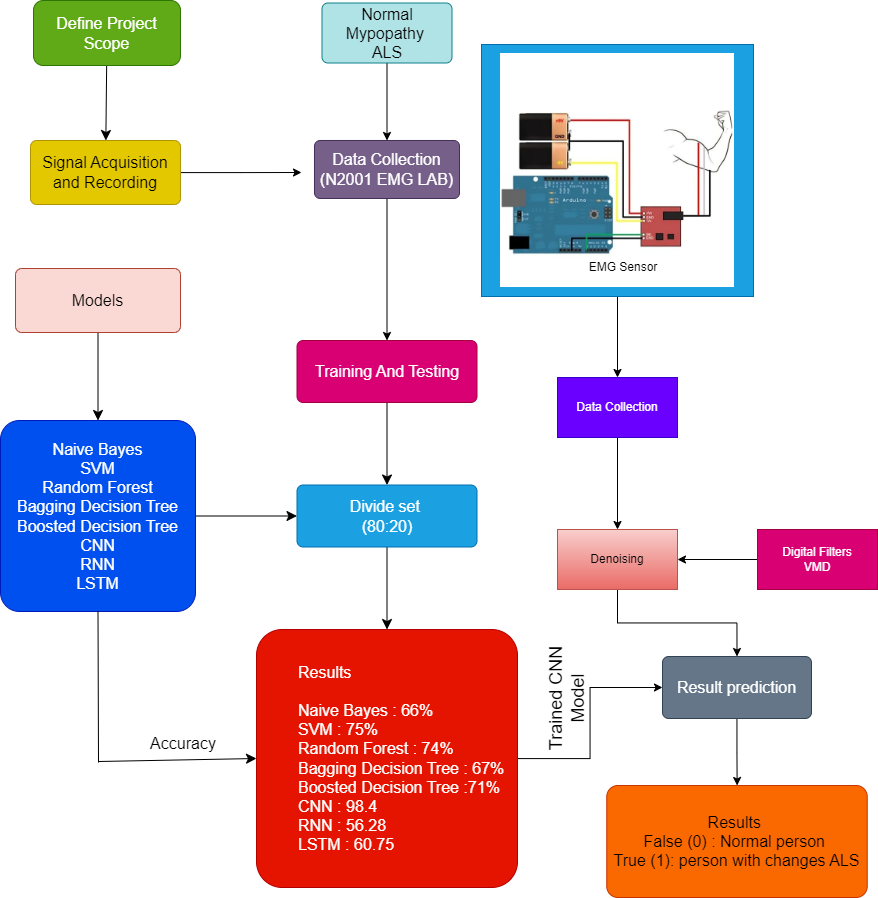
\includegraphics[width=0.7\textwidth]{image/major.png}
    \caption{Design Architecture}
    \label{fig:mesh1}
\end{figure}
\vspace{10mm}
\begin{figure}[h]
    \centering
    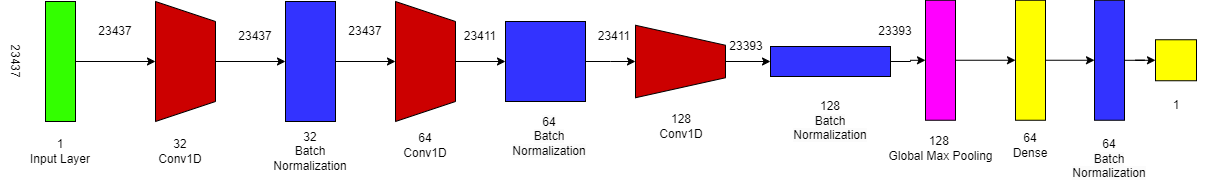
\includegraphics[width=1\textwidth]{image/CNN.png}
    \caption{CNN Architecture}
    \label{fig:mesh1}
\end{figure}
\newpage
  \pagestyle{fancy}
\thisfancypage{%
  \setlength{\fboxsep}{20pt}\doublebox}{}
\normalsize
\section{Surface Electromyography (sEMG) Electrodes}
\vspace{2mm}
Surface Electromyography (sEMG) sensors represent a non-invasive approach to measuring muscle activity, particularly suited for clinical and sports health applications. Unlike invasive methods that require electrodes to be inserted into muscles, sEMG sensors are placed directly on the skin surface, hence the "S" designation.\vskip 6pt
The non-invasive nature of sEMG sensors makes them comfortable for users, as they do not cause pain or discomfort during measurements. This quality enhances patient compliance and allows for repeated measurements without causing undue stress.\vskip 6pt
sEMG sensors find extensive use in clinical settings for diagnosing neuromuscular disorders, assessing muscle function, and monitoring rehabilitation progress. Additionally, they are prevalent in sports health applications, aiding in performance evaluation, injury prevention, and rehabilitation for athletes.\vskip 6pt
Electromyography (EMG) electrodes have historically been utilized as sensors in medical research. However, recent progress in microcontroller and integrated circuit technology has facilitated the creation of microelectrodes that are both smaller and more potent. For accurate measurement, these sensors usually necessitate the use of three electrodes that are linked to the subject's body.\vskip 6pt


\subsubsection{Brief on EMG Electrodes:} \vskip 6pt
Electromyography (EMG) electrodes play a vital role in the acquisition of electromyogram (EMG) signals, which represent the electrical activity produced by muscle contractions.
. These electrodes typically consist of pads with a diameter of 52 mm, providing sufficient surface area for accurate signal detection. To utilize EMG sensors effectively, three electrodes are required to be connected to the subject's body.\vskip 6pt
Traditionally, EMG electrodes have been extensively utilized in medical research for studying muscle function, neuromuscular disorders, and rehabilitation purposes. However, with the advancement of technology, particularly in microcontrollers and integrated circuits, EMG electrodes have found application beyond the medical field. The shrinking size and enhanced capabilities of these components have paved the way for the integration of EMG sensors into various control systems.
\newpage
  \pagestyle{fancy}
\thisfancypage{%
  \setlength{\fboxsep}{20pt}\doublebox}{}
\normalsize

\section{Placement of the Electrodes}\vskip 6pt
To effectively utilize the EMG sensor, proper placement of the electrodes on the subject's body is crucial. The following detailed guidelines outline the optimal positioning of the electrodes:\vskip 6pt
\begin{enumerate}
    \item Reference Electrode Placement:
    \begin{itemize}
    

   \item  The reference electrode serves as a baseline for measuring muscle activity and should be positioned on an inactive section of the body.
   \item  Ideal locations for the reference electrode include the bony portions of the elbow, shin, or forearm.
   \item  This electrode should be connected to either the black or brown cable of the EMG sensor.
\end{itemize}
   \item  Placement of the First Electrode:
   \begin{itemize}
   \item One of the two active electrodes should be positioned along the muscle selected for measurement.
   \item The first active electrode should be placed along the mid-length of the muscle belly.
   \item This electrode captures the electromyogram (EMG) signals generated by the muscle contractions.
   \item It should be connected to the red cable of the EMG sensor.
   \end{itemize}
\item Placement of the Second Electrode:
\begin{itemize}
   \item The second active electrode completes the trio and should be positioned at the end of the muscle being measured.
   \item This electrode captures muscle activity near the insertion point.
   \item It should be connected to the blue cable of the EMG sensor.
\end{itemize}
\item  Connection to Microcontroller:
\begin{itemize}
   \item After properly placing the electrodes, connect the EMG sensor to your microcontroller for data acquisition.
   \item Connect the pin labeled SIG (signal) to an analog input pin of your microcontroller.
   \item Connect the GND (ground) pin of the EMG sensor to the ground pin on your microcontroller.
   \item This ensures proper signal transmission and grounding for accurate measurement.
\end{itemize}

\end{enumerate}
\newpage
  \pagestyle{fancy}
\thisfancypage{%
  \setlength{\fboxsep}{20pt}\doublebox}{}
\normalsize
\begin{figure}[h]
    \centering
    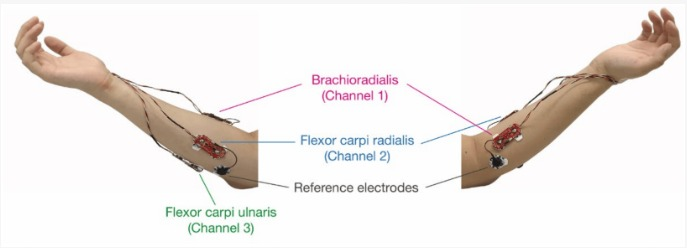
\includegraphics[width=0.98\textwidth]{image/placement.jpg}
    \caption{Placement of Electrodes}
    \label{fig:mesh1}
\end{figure}
By adhering to these guidelines, users can ensure optimal placement of EMG electrodes, facilitating accurate measurement of muscle activity for various applications ranging from medical research to control systems and beyond.

\newpage
  \pagestyle{fancy}
\thisfancypage{%
  \setlength{\fboxsep}{14pt}\doublebox}{}
\normalsize
\chapter{REQUIREMENTS}
\section{Hardware Requirements:}
\vspace{2mm}
\begin{itemize}
    \item Processor: Quad-core or higher processor (e.g., Intel Core i5, AMD Ryzen 5).
\item RAM: 16GB or higher for efficient data processing.
\item Storage: SSD with a minimum of 512GB for fast data access and storage.
\item Graphics: Dedicated GPU (NVIDIA GeForce GTX/RTX or AMD Radeon) for accelerated
machine learning computations.
\item Connectivity: High-speed internet connection for dataset retrieval and model updates.
\item Peripheral Devices:
\begin{itemize}
    \item Mouse and Keyboard: Standard input devices for system interaction.
\item Monitor: Dual monitors for efficient multitasking and data visualization.
\end{itemize}
\item Machine Learning Acceleration: If using deep learning models, consider a system with GPU
acceleration (NVIDIA CUDA-enabled GPU) to expedite model training.
\end{itemize}
\newpage
  \pagestyle{fancy}
\thisfancypage{%
  \setlength{\fboxsep}{20pt}\doublebox}{}
\normalsize
\section{Software Requirements:}
\vspace{2mm}
\begin{itemize}
    \item Python: Version 3.6 or later for coding and model development.
\item Integrated Development Environment (IDE): Choose from popular IDEs like PyCharm, Jupyter
Notebook, or Visual Studio Code.
\item Libraries and Frameworks:
\begin{itemize}
    \item TensorFlow: Open-source machine learning framework.
\item Keras: High-level neural networks API (integrated with TensorFlow).
\item Scikit-learn: Machine learning library for data preprocessing and model evaluation.
\item NumPy and Pandas: Fundamental libraries for numerical operations and data
manipulation.
\item Matplotlib and Seaborn: Visualization libraries for displaying graphs and charts
\end{itemize}
\item Machine Learning Tools:
\begin{itemize}
    \item Jupyter Notebooks: Interactive development and documentation of code and analysis.
\item TensorBoard: Visualization tool for monitoring and debugging TensorFlow models.
\item Git: Version control for collaborative development.
\end{itemize}
\item Operating System: Linux (Ubuntu or CentOS), macOS, or Windows: Choose the operating
system based on individual preferences and compatibility with required libraries.
\end{itemize}

\newpage
  \pagestyle{fancy}
\thisfancypage{%
  \setlength{\fboxsep}{20pt}\doublebox}{}
\normalsize
\chapter{EXPERIMENTATION}
\begin{itemize}
    \item Dataset Used: The project extensively utilized the EMGLAB N2001 dataset, a rich source
encompassing EMG signals from individuals with diverse characteristics. This dataset
specifically includes two primary groups: the Normal group, consisting of 10 individuals with
an age range of 21 to 37 years, and the ALS group, comprising 8 patients aged between 35 and
67 years, equally distributed between genders.
\item Exploratory Data Analysis (EDA) and Preprocessing: Through rigorous Exploratory
Data Analysis (EDA), the team gained valuable insights into the distribution of classes (Normal
vs. ALS) and delved into intricate patterns within the EMG signals. This preliminary phase laid
the foundation for effective preprocessing strategies. The data underwent meticulous
preprocessing, including standardization and normalization, ensuring uniform scaling across
features. The dataset was subsequently split into training, validation, and test sets, adhering to
an 80:20 ratio.
\item Feature Engineering and Model Selection: The project ventured into advanced feature
engineering by implementing a comprehensive four-stage signal decomposition process. This
allowed the extraction of Motor Unit Action Potentials (MUAPs) and pertinent features crucial
for ALS detection.Multiple models were explored, encompassing traditional machine learning
paradigms such as Support Vector Machines (SVM) and Random Forest, alongside deep
learning architectures like Convolutional Neural Networks (CNN), Recurrent Neural Networks
(RNN), and Long Short-Term Memory Networks (LSTM). This diversified approach aimed to
identify the most effective methodologies.
\item Training and Hyperparameter Tuning: The implementation phase involved developing
models using prevalent frameworks like TensorFlow and Keras. Models were systematically
trained, with a keen focus on hyperparameter tuning to optimize their performance. Techniques
such as grid search and random search were employed to ensure a thorough exploration of the
hyperparameter space.
\end{itemize}
\newpage
  \pagestyle{fancy}
\thisfancypage{%
  \setlength{\fboxsep}{20pt}\doublebox}{}
\normalsize
\begin{itemize}
    \item Model Evaluation and Comparison: Rigorous evaluation ensued, utilizing key
performance metrics including accuracy, precision, recall, and F1-score. Visual aids such as
Receiver Operating Characteristic (ROC) curves and precision-recall curves provided an
insightful overview of model performance. Statistical analyses were conducted to discern the
nuances in model performance, facilitating a robust comparison to identify the most accurate
and generalizable solution.
\item Model Interpretability: The team delved into the interpretability of the models, scrutinizing
feature importance to comprehend the contribution of individual features to decision-making.
For deep learning models, a layer-wise analysis was conducted, shedding light on how these
models processed input data.
\item Documentation and Reporting: A comprehensive documentation effort encapsulated the
entire journey, ranging from data preprocessing steps to intricate details of model architectures
and hyperparameters. Reports were meticulously generated, leveraging visual aids and tables to
succinctly summarize key findings and model performances.
\item Iterative Improvement and Future Directions: The project embraced a feedbackcentric approach, soliciting inputs from team members, internal project guide, and stakeholders
for ongoing improvement.
\end{itemize}
\newpage
  \pagestyle{fancy}
\thisfancypage{%
  \setlength{\fboxsep}{20pt}\doublebox}{}
\normalsize
\section{Model Selection}
\vspace{2mm}
Our investigation commenced with the utilization of machine learning models, followed by an in-depth examination of deep learning models. The primary objective of this strategy approach was to thoroughly evaluate and compare the accuracies of the models, which is a crucial step in determining the most effective model. The purpose of this thorough research was to determine the most resilient and efficient model, establishing the basis for the project's ongoing progress.
\\
\subsubsection{Naive Bayes:}
\vspace{2mm}
\begin{itemize}
    \item In our pursuit of a nuanced exploration, the Naive Bayes algorithm was chosen deliberately.
This algorithm served as the bedrock for training a machine learning model, harnessing the
potential insights embedded within the intricate EMGLAB N2001 dataset.
\item Problem Type: The specific challenge addressed here was a binary classification problem.
Naive Bayes, with its probabilistic foundation, was strategically applied to discern between two
distinct classes within the dataset.
\item Strategic Choice: The selection of Naive Bayes wasn't arbitrary but rooted in its simplicity,
computational efficiency, and adaptability to various data types. It offered a solid starting point
for our initial exploration, providing an insightful lens into the underlying patterns present in
the dataset.
\item Analytical Framework: By employing Naive Bayes, we established a foundational
understanding of the dataset. Its probabilistic approach allowed us to unravel hidden patterns
and gain valuable insights, forming the cornerstone for subsequent model comparisons.
\end{itemize}
\subsubsection{Support Vector Machine (SVM):}
\vspace{2mm}
\begin{itemize}
    \item Classifier: Our exploration extended to the sophisticated realm of Support Vector Machines
(SVM). Leveraging the Scikit-Learn library, this classifier was chosen for its robust capabilities
in handling complex datasets.
\item  Diverse Dataset Handling: SVM, renowned for its versatility, proved invaluable in handling the
intricacies of our dataset. Processing both the dataset (X\_train) and corresponding target values
(y\_train), it adeptly flattened them to a 1D array, a crucial step in optimizing model training.
\item Predictive Power: The trained SVM model emerged as a predictive powerhouse, primed to make
accurate predictions on new data. Its effectiveness in classification tasks made it an essential
contender as we delved into the comparative analysis of models.
\end{itemize}
\newpage
  \pagestyle{fancy}
\thisfancypage{%
  \setlength{\fboxsep}{20pt}\doublebox}{}
\normalsize
\subsubsection{Random Forest:}
\vspace{2mm}
\begin{itemize}
    \item Classifier: Enter the Random Forest classifier, a robust addition to our repertoire from the
Scikit-Learn library.
\item  Consistent Random State: Ensuring experimental consistency, a fixed random state was
maintained throughout. This meticulous choice allowed us to evaluate the Random Forest's
performance under controlled conditions, contributing to the robustness of our findings.
\item  Training Process: Training the model on the dataset (X\_train) and corresponding target values
(y\_train) involved careful flattening to a 1D array. This preparatory step was crucial, allowing
the Random Forest to glean insights effectively from the provided data.
\item  Versatility in Predictions: With training complete, the Random Forest model showcased its
versatility in making predictions on new, unseen data. This adaptability underscored its potential
to excel in various scenarios.
\end{itemize}
\subsubsection{Bagging Decision Tree:}
\vspace{2mm}
\begin{itemize}
    \item Effectiveness for Binary Classification: Acknowledging the nuances of binary classification,
we turned to the effectiveness of Bagging Decision Trees. This ensemble technique proved its
mettle, strategically employed to reduce variance, prevent overfitting, and enhance
generalization.
\item Ensemble of Bootstrapped Decision Trees: The model, conceived as an ensemble of
bootstrapped decision trees, underwent comprehensive training on the X\_train dataset. This
training, intertwined with corresponding target values (y\_train), epitomized a holistic approach
that harnessed collective intelligence.
\item Test Accuracy Evaluation: Moving beyond the training phase, our focus extended to evaluating
the model's performance. The culmination of this evaluation manifested in the printing of test
accuracy, providing a tangible measure of the Bagging Decision Tree's effectiveness in binary
classification tasks.
\end{itemize}
\newpage
  \pagestyle{fancy}
\thisfancypage{%
  \setlength{\fboxsep}{20pt}\doublebox}{}
\normalsize
\subsubsection{Boosted Decision Trees:}
\vspace{2mm}
\begin{itemize}
    \item Performance Improvement: The pursuit of continuous performance enhancement led us to
embrace the iterative capabilities of Boosted Decision Trees. This model, anchored on the
foundation of the DecisionTreeClassifier as the base estimator, demonstrated its prowess in
refining predictive outcomes iteratively.
\item Ensemble Method - AdaBoost: Introducing the ensemble method AdaBoost, we amalgamated
weak learners to forge a robust, strong learner. The iterative nature of boosting facilitated a
gradual improvement in model performance, particularly tailored for binary classification tasks.
\item Training Process: The ensemble, propelled by AdaBoost, underwent meticulous training on the
X\_train dataset with corresponding target values (y\_train). The flattening of target values to a
1D array facilitated a seamless integration of the Boosted Decision Trees into our comparative
analysis.

\end{itemize}
Following our initial exploration with machine learning models, we strategically transitioned to the
more sophisticated domain of deep learning models. This shift in approach was driven by the nuanced
complexities inherent in the data and the recognition that deep learning architectures possess the
capacity to discern intricate patterns and relationships that may elude conventional machine learning
models.
\begin{itemize}
    \item Sophisticated Transition: Transitioned from conventional machine learning to deep learning
models for a more sophisticated and nuanced analysis.
\item Inherent Complexity Recognition: Acknowledged the inherent complexities within the
EMGLAB N2001 dataset, prompting the shift to deep learning architectures.
\item Hierarchical Feature Extraction: Leveraged the deep learning models' ability to automatically
extract hierarchical features, providing a more nuanced understanding of complex relationships.
\item Adaptive Learning Capability: Utilized the adaptive nature of deep learning models, allowing
them to iteratively learn and refine their understanding of the data over time.
\item Intricate Pattern Recognition: Deep learning's depth facilitated the recognition of intricate
patterns, particularly crucial in medical datasets like EMGLAB N2001 for accurate diagnosis
and prediction.
\item Comparative Benchmarking: Conducted a comparative analysis of accuracies across diverse
models, serving as a critical benchmarking exercise.
\end{itemize}
\newpage
  \pagestyle{fancy}
\thisfancypage{%
  \setlength{\fboxsep}{20pt}\doublebox}{}
\normalsize
Identification of Best-Performing Model: The primary goal was to identify the best-performing
model, ensuring the selection of the most accurate and reliable approach for the project.
Insights into Dataset Dynamics: The comparative analysis not only pinpointed the optimal
model but also provided insights into the specific dataset intricacies each model excelled at
capturing.
Holistic Understanding: Achieved a holistic understanding of the dataset, essential for informed
decision-making in subsequent stages of the project.
Strategic Move for Deeper Insights: Deep learning models align with the project's goal of
gaining not only accurate predictions but deeper insights into the factors contributing to
neuromuscular disorders.
Improving Diagnostic and Predictive Capabilities: The nuanced approach of deep learning,
coupled with comparative analysis, positions the project to contribute to the improvement of
diagnostic and predictive capabilities in neuromuscular disorders.\\
\subsubsection{CNN Architecture:}
\vspace{2mm}
\begin{itemize}
    \item Input Layer: Defines the input shape of the data. Shape determined by the number of time steps
(X\_train.shape[1]) and features per time step (X\_train.shape[2]).
\item Convolutional Layers (conv1, conv2, conv3): 1D convolutional layers capturing patterns in
input data. Different parameters (filters, kernel size, dilation rate, activation function). Each
followed by batch normalization (conv1\_bn, conv2\_bn, conv3\_bn) for stability.
\item Global Max Pooling Layer (Max\_pool): GlobalMaxPooling1D reduces spatial dimensions by
taking the maximum value along the time axis. Captures crucial features from convolutional
layers.
\item Dense Layers (Emg\_block): Dense layer with ReLU activation and batch normalization.
Processes output from the global max pooling layer.
\item Final Layer (Emg): Dense layer with sigmoid activation for binary classification output.
\item Model Compilation: Compiled using Adam optimizer with specified learning rate. Binary crossentropy loss function used, and no additional metrics included.
\end{itemize}
\newpage
  \pagestyle{fancy}
\thisfancypage{%
  \setlength{\fboxsep}{20pt}\doublebox}{}
\normalsize
\subsubsection{RNN Architecture:}
\vspace{2mm}
\begin{itemize}
    \item Initialize RNN (Recurrent Neural Network): Sequential model for layer-by-layer neural network
construction.
\item Add the First RNN Layer: SimpleRNN layer with 32 units (neurons). Processes input sequences,
returns sequences (return\_sequences=True). Uses hyperbolic tangent (tanh) activation and
dropout regularization (rate of 0.2) to prevent overfitting.
\item Add the Second RNN Layer: Second SimpleRNN layer with the same configuration as the first.
Returns sequences and includes dropout regularization.
\item Add the Output Layer: Dense layer with one unit and sigmoid activation. Suitable for binary
classification, squashing output between 0 and 1.
\item Compile the RNN: Compiled using Adam optimizer. Binary cross-entropy loss chosen for
binary classification problems. Accuracy used as the evaluation metric.

\end{itemize}
\subsubsection{LSTM Architecture:}
\vspace{2mm}
\begin{itemize}
    \item Define the LSTM Model: Sequential model for layer-by-layer construction.
\item Add the LSTM Layer: LSTM layer responsible for capturing sequential dependencies. Defined
by the number of memory cells or LSTM units (set to 50 in this example). Input shape defined
by X.shape[1] (length of each sequence) and X.shape[2] (number of features at each time step).
\item Add the Dense Output Layer: Dense layer for final classification with one unit and sigmoid
activation. Output between 0 and 1, representing the probability of belonging to the positive
class.
\item Compile the Model: Compiled using the Adam optimizer, an adaptive learning rate algorithm.
Binary cross-entropy loss selected for binary classification problems. Accuracy monitored
during training.
\item Training Details: Training performed for 10 epochs, going through the entire dataset 10 times.
Batch size set to 32, updating weights after processing 32 samples.
\end{itemize}
\newpage
  \pagestyle{fancy}
\thisfancypage{%
  \setlength{\fboxsep}{20pt}\doublebox}{}
\normalsize
\section{Working of SEMG Sensors}\vskip 6pt
An EMG sensor, or electromyography sensor, is designed to measure the small electrical signals generated by muscles when they are activated or moved. The process of muscle activation and signal detection involves several steps:
\begin{figure}[h]
    \centering
    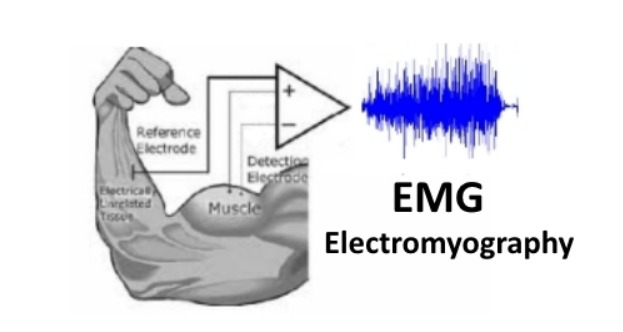
\includegraphics[width=0.5\textwidth]{image/muscel.jpg}
    \caption{Working of SEMG}
    \label{fig:mesh1}
\end{figure}
\begin{enumerate}
    \item  Neural Signaling from the Brain:
   The process begins in the brain, specifically in the motor cortex, which is responsible for initiating voluntary muscle movements. When you decide to move a muscle, signals are sent from the motor cortex through neural pathways to the spinal cord.


\item Transmission of Signals via Motor Neurons:
In the spinal cord, the signals are transmitted via motor neurons, specialized nerve cells that extend from the spinal cord to the muscles. These motor neurons carry the neural impulses from the spinal cord to the target muscle.

\item Muscle Activation and Calcium Release:
   Upon receiving signals from the motor neurons, the muscle fibers within the target muscle are activated. This activation triggers the release of calcium ions within the muscle cells.

\item Electromechanical Changes:
   The release of calcium ions within the muscle cells leads to a series of biochemical reactions that result in depolarization, or a change in the electromechanical gradient across the cell membrane. This depolarization causes the muscle fibers to contract, generating mechanical force and movement.

\item Detection by EMG Sensors:
   The mechanical changes associated with muscle activation, including depolarization and contraction, produce electrical signals known as electromyograms (EMGs). EMG sensors are designed to detect and measure these electrical signals. They typically consist of electrodes placed on the surface of the skin or inserted into the muscle tissue. As the muscle contracts and generates electrical activity, the EMG sensor picks up these signals and converts them into measurable data.

\end{enumerate}
\newpage
  \pagestyle{fancy}
\thisfancypage{%
  \setlength{\fboxsep}{20pt}\doublebox}{}
\normalsize
EMG sensors work by detecting the electrical signals generated by muscles during contraction. This process involves the initiation of neural signals in the brain, transmission through the spinal cord and motor neurons, muscle activation and calcium release, and ultimately, the detection of electromyographic signals by the EMG sensor.
\subsection{Sample EMG Sensor Output}\vskip 6pt
\begin{figure}[h]
    \centering
    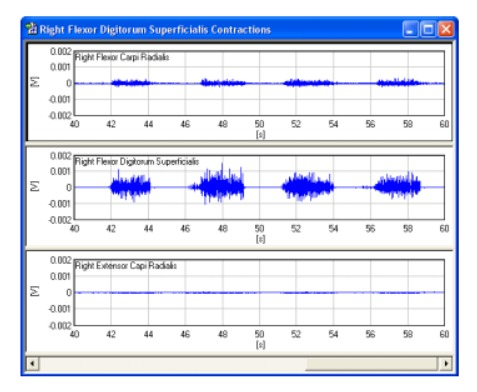
\includegraphics[width=0.5\textwidth]{image/sensor_reading.jpg}
    \caption{Sample Sensor Output}
    \label{fig:mesh1}
\end{figure}
By accurately capturing and analyzing electrical activity at the surface level, EMG sensors offer a non-invasive and effective means of assessing neuromuscular function, facilitating diagnostics, rehabilitation, and performance enhancement across various fields, including healthcare, sports science, and ergonomics.

\subsection{How Surface EMG Sensors Work}\vskip 6pt
Surface Electromyography (sEMG) sensors are instrumental in capturing and analyzing muscle activity, providing valuable insights into motor function and performance. The following steps elucidate the working principle of surface EMG sensors:
\begin{enumerate}
    \item Placement of EMG Sensors:
    \begin{itemize}
\item 	Surface EMG sensors are strategically placed on the skin surface, typically within the innervation zone of relevant muscles or overlying tendons for optimal signal detection.
\item 	Proper placement ensures closer proximity to muscle fibers, enhancing the quality and accuracy of signal acquisition.

\end{itemize}
\newpage
  \pagestyle{fancy}
\thisfancypage{%
  \setlength{\fboxsep}{20pt}\doublebox}{}
\normalsize
\item	Placement of EMG Sensors:
\begin{itemize}
\item	Surface EMG sensors are strategically placed on the skin surface, typically within the innervation zone of relevant muscles or overlying tendons for optimal signal detection.
\item	Proper placement ensures closer proximity to muscle fibers, enhancing the quality and accuracy of signal acquisition.
\end{itemize}
\item	Signal Processing and Visualization:
\begin{itemize}
\item	The detected electrical activity is processed and amplified by the surface EMG sensor to enhance signal clarity and resolution.
\item	The processed EMG signals are then displayed in real-time on a monitor, often in the form of waveforms.
\item	This visualization allows clinicians, researchers, or users to observe and analyze the characteristics of muscle activity, including amplitude, frequency, and duration.
\end{itemize}
\item	Interpretation and Analysis:
\begin{itemize}
\item	The displayed EMG waveforms provide valuable information regarding muscle activation patterns, timing, and coordination.
\item	Clinicians and researchers can interpret these signals to assess muscle function, diagnose neuromuscular disorders, evaluate rehabilitation progress, or optimize performance in sports and exercise science.
\end{itemize}
\item	Feedback and Adjustment:
\begin{itemize}
\item	Surface EMG sensors may provide real-time feedback to users, facilitating biofeedback training or neuromuscular re-education.
\item	Based on the observed EMG patterns, users can adjust their movements or exercises to optimize muscle recruitment, coordination, and performance.
\end{itemize}
\end{enumerate}
\subsection{Addressing Challenges in sEMG Analysis}\vskip 6pt
Although sEMG has the potential to diagnose neuromuscular diseases, it encounters various obstacles in this context:
\newpage
  \pagestyle{fancy}
\thisfancypage{%
  \setlength{\fboxsep}{20pt}\doublebox}{}
\normalsize
\begin{itemize}
    \item sEMG noise can be caused by various factors such as electrode
placement mistakes, motion artifacts, muscle interference, and
other electrical sources. The presence of background noise obscures the patterns of neuromuscular activity, hence complicating the diagnosis of illnesses.
\item Cross-talk occurs when electrodes detect signals emitted by
adjacent muscles, resulting in the contamination of the sEMG
signal. The presence of this interference might provide difficulties in data interpretation, particularly when the target muscles
are in close proximity.
\item Signal Variability The amplitude and frequency of sEMG signals can exhibit significant variations due to factors such as
muscle fatigue, electrode properties, and subject-to-subject
changes. The presence of variability poses challenges in the
development of neuromuscular disease diagnosis algorithms
\end{itemize}
The utilization of convolutional neural networks (CNNs)[19] and
other sophisticated signal processing and machine learning techniques has been investigated as a potential option for the analysis
of SEMG data.Convolutional neural networks (CNNs) can readily
identify spatial and temporal patterns in sequential data, such as
sEMG signals. 1D dilated convolutional layers enable the network
to record patterns at various temporal scales, hence facilitating the
extraction of supplementary information.\\

Aside from CNN layers, the application of low-pass and high-pass
filtering enhances the quality of sEMG data prior to its input into
the network.\\

In sEMG signals, a high-pass filter is employed to eliminate baseline and low-frequency drift. Preprocessing eliminates undesired
elements and standardizes the signal, enhancing the precision of
disease detection.\\

Low-pass filtering is employed to eliminate high-frequency noise
and artifacts from the simultaneous electromyography (sEMG) signal, while maintaining the fundamental neuromuscular activity.
This technique contributes to the enhancement of the signal-tonoise ratio and improves the network’s capacity to retrieve pertinent features.
\newpage
  \pagestyle{fancy}
\thisfancypage{%
  \setlength{\fboxsep}{20pt}\doublebox}{}
\normalsize
\chapter{RESULT AND ANALYSIS}
An in-depth analysis underscores the unique advantages each model brings to the table. While CNN
excels in spatial feature extraction, RNN specializes in sequential dependencies, and LSTM further
refines long-term memory retention. The comparative study enriches our understanding, guiding the
selection of the most suitable model for the project's nuanced requirements is CNN.
\begin{figure}[h]
    \centering
    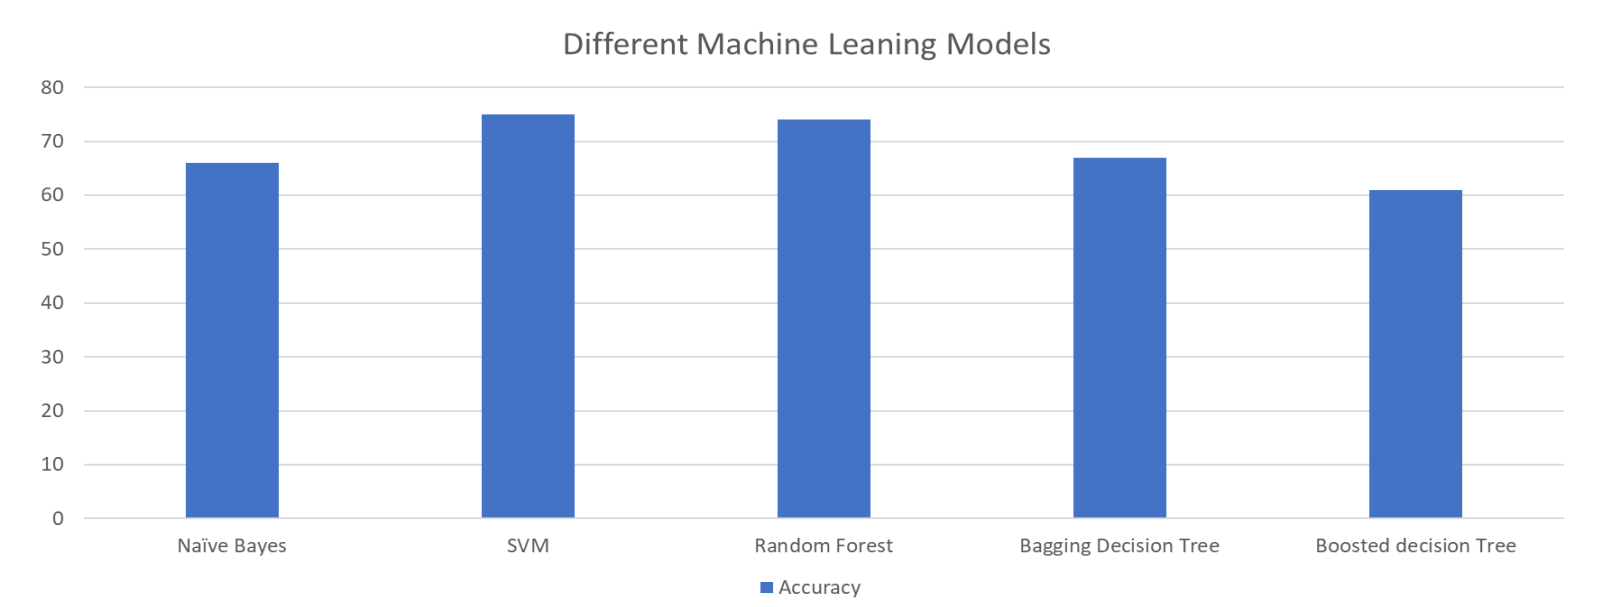
\includegraphics[width=0.98\textwidth]{image/result1.png}
    \caption{Graph Displaying Accuracy of Different Machine Learning Models}
    \label{fig:mesh1}
\end{figure}

From the above fig 7.1 we observe that the accuracy of various different machine learning models lies
in a range of 66 \% to 75\% which naïve bayes bring the lowest accuracy model and SVM providing the
highest of the accuracy
\newpage
  \pagestyle{fancy}
\thisfancypage{%
  \setlength{\fboxsep}{20pt}\doublebox}{}
\normalsize
\begin{table}[]
    \centering
    \begin{tabular}{|c|c|}
    \hline
     MACHINE LEARNING MODELS & MODELS ACCURACY \\
   \hline
   NAÏVE BAYES & 66 \% \\
   \hline
   SUPPORT VERCTOR MACHINE & 75 \%\\
    \hline
    RANDOM FOREST & 74 \% \\
    \hline
    BAGGING DECISION TREE & 67 \%\\
    \hline
    BOOSTED DECISION TREE & 71 \% \\
    \hline
    \end{tabular}
    \caption{Accuracy of different machine learning models}
    \label{tab:my_label}
\end{table}
The figure fig 7.2 shows the graphical representation of accuracy of different deep learning models
applied which the accuracy ranging from 56 \% - 98.4 \% where the model RNN performed the lowest
among all 3 models and our purposed CNN model performed the highest of 98.4 \% standing ahead of
all the models applied\\
\begin{figure}[h]
    \centering
    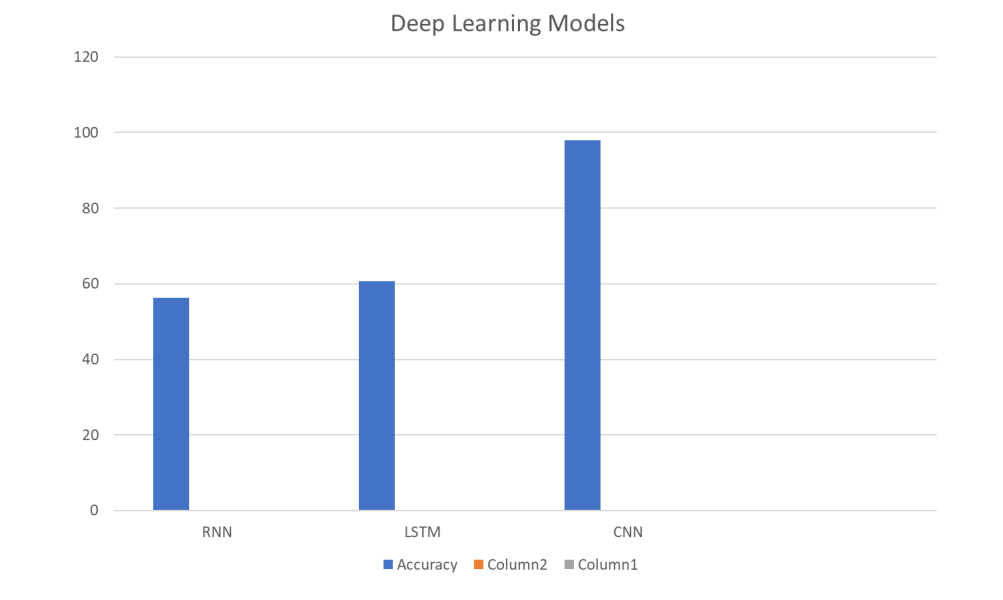
\includegraphics[width=0.98\textwidth]{image/result2.png}
    \caption{Graph Displaying Accuracy of Different Deep learning Models Learning Models}
    \label{fig:mesh1}
\end{figure}
\newpage
  \pagestyle{fancy}
\thisfancypage{%
  \setlength{\fboxsep}{20pt}\doublebox}{}
\normalsize
\begin{table}[]
    \centering
    \begin{tabular}{|c|c|}
    \hline
     DEEP LEARNING MODELS & MODELS ACCURACY \\
   \hline
   RNN & 56.28 \% \\
   \hline
   LSTM & 60.75 \%\\
    \hline
    CNN & 98.4 \% \\

    \hline
    \end{tabular}
    \caption{Accuracy of different Deep learning models}
    \label{tab:my_label}
\end{table}
The CNN model provided the best results of 98.4\% over throwing all the models the below fig 7.3
shows the model loss vs epoch graph which gives an idea of how good our model has performed . The
Figure 7.4 shows the results from the different accuracy matrices results given by the CNN model.
\begin{figure}[h]
    \centering
    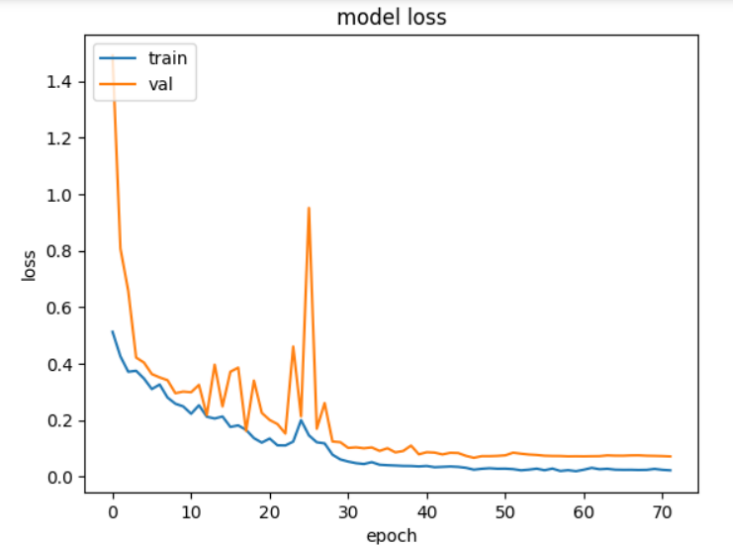
\includegraphics[width=0.65\textwidth]{image/result3.png}
    \caption{Model loss vs epoch}
    \label{fig:mesh1}
\end{figure}
\vspace{10mm}
\begin{figure}[h]
    \centering
    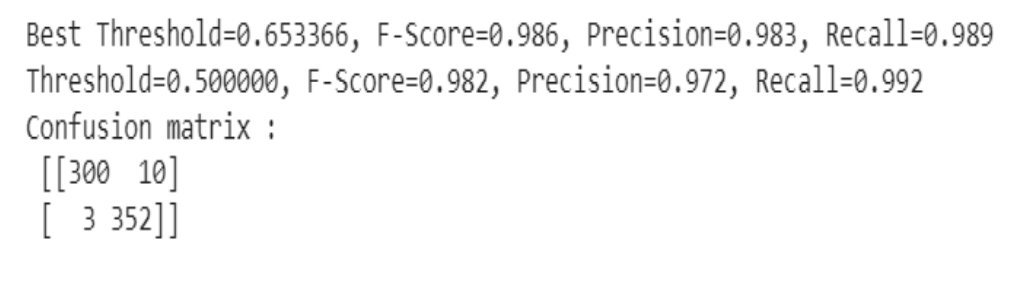
\includegraphics[width=0.8\textwidth]{image/result4.png}
    \caption{Accuracy Matrix of CNN Model}
    \label{fig:mesh1}
\end{figure}
\newpage
  \pagestyle{fancy}
\thisfancypage{%
  \setlength{\fboxsep}{20pt}\doublebox}{}
\normalsize
\chapter{CONCLUSION AND FUTURE SCOPE}
A Convolutional Neural Network (CNN) model trained on N2001
EMGlab data was identified, marking a major milestone for the
study. This model boasts an amazing accuracy rate of around 98.4
percent for the categorization of ALS. This represents a significant
step forward in the area, demonstrating the promise of using advanced machine learning methods for early ALS detection. Using
surface electromyography (EMG) data collected from easily accessible EMG electrodes for real-time prediction is the main focus at
the moment. Further evaluation and refinement are necessary to optimize the model’s performance in this environment, although initial attempts have showed promise.\\
This study’s findings have far-reaching consequences because they
demonstrate the promise of combining easily accessible surface
EMG data with cutting-edge machine learning models. This convergence shows great potential for changing the way amyotrophic
lateral sclerosis (ALS) is diagnosed. By detecting the disease early
on, patient outcomes can be greatly improved and disease management measures can be more effective. This discovery opens the
door to a proactive strategy for amyotrophic lateral sclerosis (ALS)
detection and management through the use of cutting-edge technology, which gives individuals impacted by the disease hope for an
enhanced quality of life. The culmination of this phase prompts a detailed reflection on our
achievements and sets the stage for future explorations.\\
\begin{itemize}
    \item Efficient Signal Decomposition: The systematic approach to EMG signal decomposition,
encompassing stages of filtering, segmentation, clustering, and resolution, has proven to be a
robust framework for identifying Motor Unit Action Potentials (MUAPs) and decoding intricate
patterns of neuromuscular activity.
\item Practicality of Surface Electrodes: The choice of surface electrodes not only aligns with
practical usability but also ensures a minimally invasive yet reliable method for capturing EMG
signals. This consideration enhances the real-world applicability of our methodology.
\newpage
  \pagestyle{fancy}
\thisfancypage{%
  \setlength{\fboxsep}{20pt}\doublebox}{}
\normalsize
\item Dataset Selection and Diversity: The strategic selection of the EMGLAB N2001 dataset,
focusing on both Normal and ALS groups, has facilitated a comprehensive understanding of
diverse neuromuscular activities. The dataset's age and gender diversity contribute to the
richness of our model training.
\item Holistic Approach to Diagnosis: By integrating surface electrodes and a systematic signal
processing methodology, our project takes a holistic approach to neuromuscular disorder
diagnosis. This not only aids in early ALS detection but also sets the foundation for future
advancements in the field.
\end{itemize}

\section{Implications and Future Directions:}
\vspace{2mm}
\begin{itemize}
    \item Dataset Expansion Strategy: The planned expansion of our dataset collection, targeting normal
individuals and those diagnosed with ALS, signifies a forward-thinking approach. This
expansion is poised to fortify our machine learning models, ensuring their adaptability to a
broader range of neuromuscular conditions.
Model Refinement and Iteration: Future iterations of our machine learning models will involve
continuous refinement based on insights gained from ongoing experimentation. Exploring
advanced architectures and techniques will contribute to the evolution of accurate and reliable
ALS detection models.
\item Real-time Application and Clinical Integration: Transitioning our models for real-time
application, especially in clinical settings, holds immense potential. This could pave the way
for swift and accurate diagnosis, enabling timely interventions and improved patient outcomes.

\item Multimodal Integration: Exploring the integration of additional diagnostic markers, such as
genetic information or clinical data, can enhance the comprehensiveness of our diagnostic
models. This multimodal approach may uncover nuanced correlations, further improving
diagnostic accuracy.
\item Collaboration and Ethical Considerations: Collaborative efforts with healthcare professionals
will be instrumental in guiding the practical application of our models. Emphasis on ethical
considerations, patient consent, and data privacy will remain central to the responsible
development and deployment of diagnostic tools.
\end{itemize}

\vspace{2mm}
In conclusion, our detailed exploration and application of EMG signal analysis for ALS detection
underscore the potential for groundbreaking advancements in neuromuscular disorder diagnostics. The
achievements to date, coupled with the strategic vision for the future, position our project at the
forefront of innovation in the quest for early detection and intervention in ALS and related disorders
\newpage
  \pagestyle{fancy}
\thisfancypage{%
  \setlength{\fboxsep}{20pt}\doublebox}{}
\normalsize
\section{Future Scope}
\vspace{4mm}
\begin{itemize}
    \item Understanding Neuromuscular Diseases: Dive into literature and online resources to grasp the
fundamentals of neuromuscular diseases, including their impact on motor functions. Explore
educational platforms offering insights into the neurological aspects of conditions like ALS.
\item Online Courses and Webinars: Enroll in online courses and webinars focusing on the
intersection of neuroscience, EMG technology, and prosthetic solutions. Participate in virtual
lectures by professionals in the field to deepen knowledge.
\end{itemize}

\begin{itemize}
    \item Small-Scale Projects: Undertake small-scale projects applying EMG technology to understand
how neuromuscular diseases affect muscle activity. Collaborate with peers on projects related
to the classification of EMG signals in the context of muscle disorders.
\item Research Initiatives: Explore research articles and case studies related to the use of EMG in
diagnosing and understanding neuromuscular diseases. Experiment with EMG signal
processing techniques on open-access datasets to gain practical insights.
\item Simulating Neuromuscular Conditions: Utilize open-source simulation software to recreate
conditions akin to neuromuscular diseases. Develop virtual environments that simulate
challenges faced by individuals with impaired motor functions.
\item Community Engagement: Engage with online communities focused on both neuromuscular
diseases and DIY prosthetics. Seek advice from individuals who have experience with EMG
technology in the context of neurological disorders.

\item Iterative Design with Neurological Considerations: Integrate considerations for muscle
weakness, spasticity, or atrophy into the design of the prosthetic limb. Iteratively modify the
hardware prototype to address challenges related to neuromuscular conditions.
\item User-Centric Approach: Connect with local support groups for individuals affected by
neuromuscular diseases. Conduct user trials to gather feedback on the practicality and
adaptability of the DIY EMG-controlled prosthetic limb in real-world scenarios.
\item Knowledge Sharing: Document the journey of developing a neuromuscular-aware prosthetic
limb, emphasizing challenges unique to this context. Share findings through online platforms,
contributing to the knowledge base of DIY solutions for neuromuscular disorders.
\end{itemize}
\newpage
  \pagestyle{fancy}
\thisfancypage{%
  \setlength{\fboxsep}{20pt}\doublebox}{}
\begin{center}

    \huge\textbf{REFERENCES}
\end{center}
\vspace{10mm}
\normalsize
[1] T. Ahmed and M. K. Islam, "EMG Signal Classification for Detecting Neuromuscular Disorders,"
J. Phys.: Conf. Ser., vol. 1921, p. 012043, 2021, DOI: 10.1088/1742-6596/1921/1/012043.
\\
\hfill
[2] A. Phinyomark, P. Phukpattaranont, and C. Limsakul, "Feature reduction and selection for EMG
signal classification," Department of Electrical Engineering, Faculty of Engineering, Prince of Songkla
University.
\\
\hfill
[3] A. Mokdad, S. M. E. Amine Debba, and F. Meziani, "Diagnosis of amyotrophic lateral sclerosis
(ALS) disorders based on electromyogram (EMG) signal analysis and feature selection," Polish Journal
of Medical Physics and Engineering, vol. 26, no. 3, Sep. 2020, DOI: 10.2478/pjmpe-2020-0018.
\\
\hfill
[4] P. Kaplanis, C. S. Pattichis, L. Hadjileontiadis, and S. M. Panas, "Bispectral analysis of surface
EMG," in Proceedings of the IEEE Mediterranean Electrotechnical Conference (MELCON), February
2000, DOI: 10.1109/MELCON.2000.880047.
\\
\hfill
[5] A. Alkan and M. Günay, "Identification of EMG signals using discriminant analysis and SVM
classifier," Kahramanmaras Sutcu Imam University, Department of Electrical \& Electronics
Engineering.
\\
\hfill
[6] Mayo Clinic, "Amyotrophic Lateral Sclerosis (ALS) - Symptoms and Causes,"\\
www.mayoclinic.org/diseases-conditions/amyotrophic-lateral-sc.
\\
\hfill
[7] "Machine Learning | Detection of ALS | Amyotrophic Lateral Sclerosis | EMG," YouTube,
https://youtu.be/UOf3dkOiJz8?si=-AVjQsmuha1Vp6zr.
\\
\hfill
[8] "Amyotrophic Lateral Sclerosis (ALS)," National Institute of Neurological Disorders and Stroke,
www.ninds.nih.gov/health-information/disorders/\\
amyotrophic-lateral-sclerosisals\#:~:text=Although\%20not\%20as\%20common\%2C\%20people.
\\
\hfill
[9] V. Kehri, R. Ingle, R. Awale, and S. Oimbe, “Techniques of EMG signal analysis and classification
of neuromuscular diseases,” www.atlantis-press.com, Dec. 01, 2016. \\https://www.atlantispress.com/proceedings/iccasp-16/25871652.
\\
\hfill
[10] M. J. Zwarts, G. Drost, and D. F. Stegeman, “Recent progress in the diagnostic use of surface
EMG for neurological diseases,” Journal of Electromyography and Kinesiology, vol. 10, no. 5, pp.
287–291, Oct. 2000, doi: https://doi.org/10.1016/s1050-6411(00)00020-1.
\\
\hfill
[11] Anjana Goen, "Classification of EMG Signals for Assessment of Neuromuscular Disorders,"
International Journal of Electronics and Electrical Engineering, Vol. 2, No. 3, pp. 242-248, September
2014. doi: 10.12720/ijeee.2.3.242-248


\end{document}